\documentclass[]{article}
\usepackage{lmodern}
\usepackage{amssymb,amsmath}
\usepackage{ifxetex,ifluatex}
\usepackage{fixltx2e} % provides \textsubscript
\ifnum 0\ifxetex 1\fi\ifluatex 1\fi=0 % if pdftex
  \usepackage[T1]{fontenc}
  \usepackage[utf8]{inputenc}
\else % if luatex or xelatex
  \ifxetex
    \usepackage{mathspec}
    \usepackage{xltxtra,xunicode}
  \else
    \usepackage{fontspec}
  \fi
  \defaultfontfeatures{Mapping=tex-text,Scale=MatchLowercase}
  \newcommand{\euro}{€}
\fi
% use upquote if available, for straight quotes in verbatim environments
\IfFileExists{upquote.sty}{\usepackage{upquote}}{}
% use microtype if available
\IfFileExists{microtype.sty}{%
\usepackage{microtype}
\UseMicrotypeSet[protrusion]{basicmath} % disable protrusion for tt fonts
}{}
\ifxetex
  \usepackage[setpagesize=false, % page size defined by xetex
              unicode=false, % unicode breaks when used with xetex
              xetex]{hyperref}
\else
  \usepackage[unicode=true]{hyperref}
\fi
\hypersetup{breaklinks=true,
            bookmarks=true,
            pdfauthor={},
            pdftitle={},
            colorlinks=true,
            citecolor=blue,
            urlcolor=blue,
            linkcolor=magenta,
            pdfborder={0 0 0}}
\urlstyle{same}  % don't use monospace font for urls
\usepackage{color}
\usepackage{fancyvrb}
\newcommand{\VerbBar}{|}
\newcommand{\VERB}{\Verb[commandchars=\\\{\}]}
\DefineVerbatimEnvironment{Highlighting}{Verbatim}{commandchars=\\\{\}}
% Add ',fontsize=\small' for more characters per line
\newenvironment{Shaded}{}{}
\newcommand{\KeywordTok}[1]{\textcolor[rgb]{0.00,0.44,0.13}{\textbf{{#1}}}}
\newcommand{\DataTypeTok}[1]{\textcolor[rgb]{0.56,0.13,0.00}{{#1}}}
\newcommand{\DecValTok}[1]{\textcolor[rgb]{0.25,0.63,0.44}{{#1}}}
\newcommand{\BaseNTok}[1]{\textcolor[rgb]{0.25,0.63,0.44}{{#1}}}
\newcommand{\FloatTok}[1]{\textcolor[rgb]{0.25,0.63,0.44}{{#1}}}
\newcommand{\ConstantTok}[1]{\textcolor[rgb]{0.53,0.00,0.00}{{#1}}}
\newcommand{\CharTok}[1]{\textcolor[rgb]{0.25,0.44,0.63}{{#1}}}
\newcommand{\SpecialCharTok}[1]{\textcolor[rgb]{0.25,0.44,0.63}{{#1}}}
\newcommand{\StringTok}[1]{\textcolor[rgb]{0.25,0.44,0.63}{{#1}}}
\newcommand{\VerbatimStringTok}[1]{\textcolor[rgb]{0.25,0.44,0.63}{{#1}}}
\newcommand{\SpecialStringTok}[1]{\textcolor[rgb]{0.73,0.40,0.53}{{#1}}}
\newcommand{\ImportTok}[1]{{#1}}
\newcommand{\CommentTok}[1]{\textcolor[rgb]{0.38,0.63,0.69}{\textit{{#1}}}}
\newcommand{\DocumentationTok}[1]{\textcolor[rgb]{0.73,0.13,0.13}{\textit{{#1}}}}
\newcommand{\AnnotationTok}[1]{\textcolor[rgb]{0.38,0.63,0.69}{\textbf{\textit{{#1}}}}}
\newcommand{\CommentVarTok}[1]{\textcolor[rgb]{0.38,0.63,0.69}{\textbf{\textit{{#1}}}}}
\newcommand{\OtherTok}[1]{\textcolor[rgb]{0.00,0.44,0.13}{{#1}}}
\newcommand{\FunctionTok}[1]{\textcolor[rgb]{0.02,0.16,0.49}{{#1}}}
\newcommand{\VariableTok}[1]{\textcolor[rgb]{0.10,0.09,0.49}{{#1}}}
\newcommand{\ControlFlowTok}[1]{\textcolor[rgb]{0.00,0.44,0.13}{\textbf{{#1}}}}
\newcommand{\OperatorTok}[1]{\textcolor[rgb]{0.40,0.40,0.40}{{#1}}}
\newcommand{\BuiltInTok}[1]{{#1}}
\newcommand{\ExtensionTok}[1]{{#1}}
\newcommand{\PreprocessorTok}[1]{\textcolor[rgb]{0.74,0.48,0.00}{{#1}}}
\newcommand{\AttributeTok}[1]{\textcolor[rgb]{0.49,0.56,0.16}{{#1}}}
\newcommand{\RegionMarkerTok}[1]{{#1}}
\newcommand{\InformationTok}[1]{\textcolor[rgb]{0.38,0.63,0.69}{\textbf{\textit{{#1}}}}}
\newcommand{\WarningTok}[1]{\textcolor[rgb]{0.38,0.63,0.69}{\textbf{\textit{{#1}}}}}
\newcommand{\AlertTok}[1]{\textcolor[rgb]{1.00,0.00,0.00}{\textbf{{#1}}}}
\newcommand{\ErrorTok}[1]{\textcolor[rgb]{1.00,0.00,0.00}{\textbf{{#1}}}}
\newcommand{\NormalTok}[1]{{#1}}
\usepackage{graphicx,grffile}
\makeatletter
\def\maxwidth{\ifdim\Gin@nat@width>\linewidth\linewidth\else\Gin@nat@width\fi}
\def\maxheight{\ifdim\Gin@nat@height>\textheight\textheight\else\Gin@nat@height\fi}
\makeatother
% Scale images if necessary, so that they will not overflow the page
% margins by default, and it is still possible to overwrite the defaults
% using explicit options in \includegraphics[width, height, ...]{}
\setkeys{Gin}{width=\maxwidth,height=\maxheight,keepaspectratio}
\setlength{\parindent}{0pt}
\setlength{\parskip}{6pt plus 2pt minus 1pt}
\setlength{\emergencystretch}{3em}  % prevent overfull lines
\providecommand{\tightlist}{%
  \setlength{\itemsep}{0pt}\setlength{\parskip}{0pt}}
\setcounter{secnumdepth}{0}

\date{}

% Redefines (sub)paragraphs to behave more like sections
\ifx\paragraph\undefined\else
\let\oldparagraph\paragraph
\renewcommand{\paragraph}[1]{\oldparagraph{#1}\mbox{}}
\fi
\ifx\subparagraph\undefined\else
\let\oldsubparagraph\subparagraph
\renewcommand{\subparagraph}[1]{\oldsubparagraph{#1}\mbox{}}
\fi

\begin{document}

\section{Goal}\label{goal}

\textbf{\emph{In this chapter:}}\\
* We will learn how to detect the marker\\
* We will learn how to determine the distance, angle of the marker with respect to the camera\\
* We will learn how to map the real world coordinates on to a virtual arena \\
* We will learn about socket programming

\section{Pre-requisites}\label{pre-requisites}

\begin{itemize}
\tightlist
\item
  \href{https://github.com/eyantrainternship/eYSIP_2015_Marker_based_Robot_Localisation/wiki/ArUco-Markers}{Aruco
  markers}
\item
  \href{https://www.google.co.in/url?sa=t\&rct=j\&q=\&esrc=s\&source=web\&cd=5\&ved=0CDYQFjAE\&url=https\%3A\%2F\%2Fen.wikipedia.org\%2Fwiki\%2FHamming_distance\&ei=BE6cVcWyEoaJuwTB94LgDA\&usg=AFQjCNFSM3VMSv1QOWQPVYax0JHs_yf5Ww\&sig2=TZGcg4nvTEBwxxL35O0ycQ}{Hamming
  distance}
\item
  \href{https://github.com/eyantrainternship/eYSIP_2015_Marker_based_Robot_Localisation/wiki/Camera-Calibration}{Camera
  Calibration}
\item
  \href{https://github.com/eyantrainternship/eYSIP_2015_Marker_based_Robot_Localisation/wiki/Pose-Estimation}{Pose
  estimation}
\item
  \href{https://www.google.co.in/url?sa=t\&rct=j\&q=\&esrc=s\&source=web\&cd=1\&cad=rja\&uact=8\&ved=0CB4QFjAA\&url=http\%3A\%2F\%2Fmobaxterm.mobatek.net\%2F\&ei=nU-cVaetMc22uAT8w4OgDA\&usg=AFQjCNFIes6M8iS_0iHFNFymtm-GbRSZow\&sig2=fywu_0EqUwUPuvxFg2kVMQ}{SSH
  - MobaXterm}
\end{itemize}

\section{Construction}\label{construction}

The Raspberry pi (Raspi) will be mounted on top of the Firebird V robot.
To power the Raspi we will use a power bank. For additional power to the
Raspi, GPIO pins can be used. An USB webcam will be connected to the USB
port of the Raspi.\\
Finally the setup should look like this:\\
 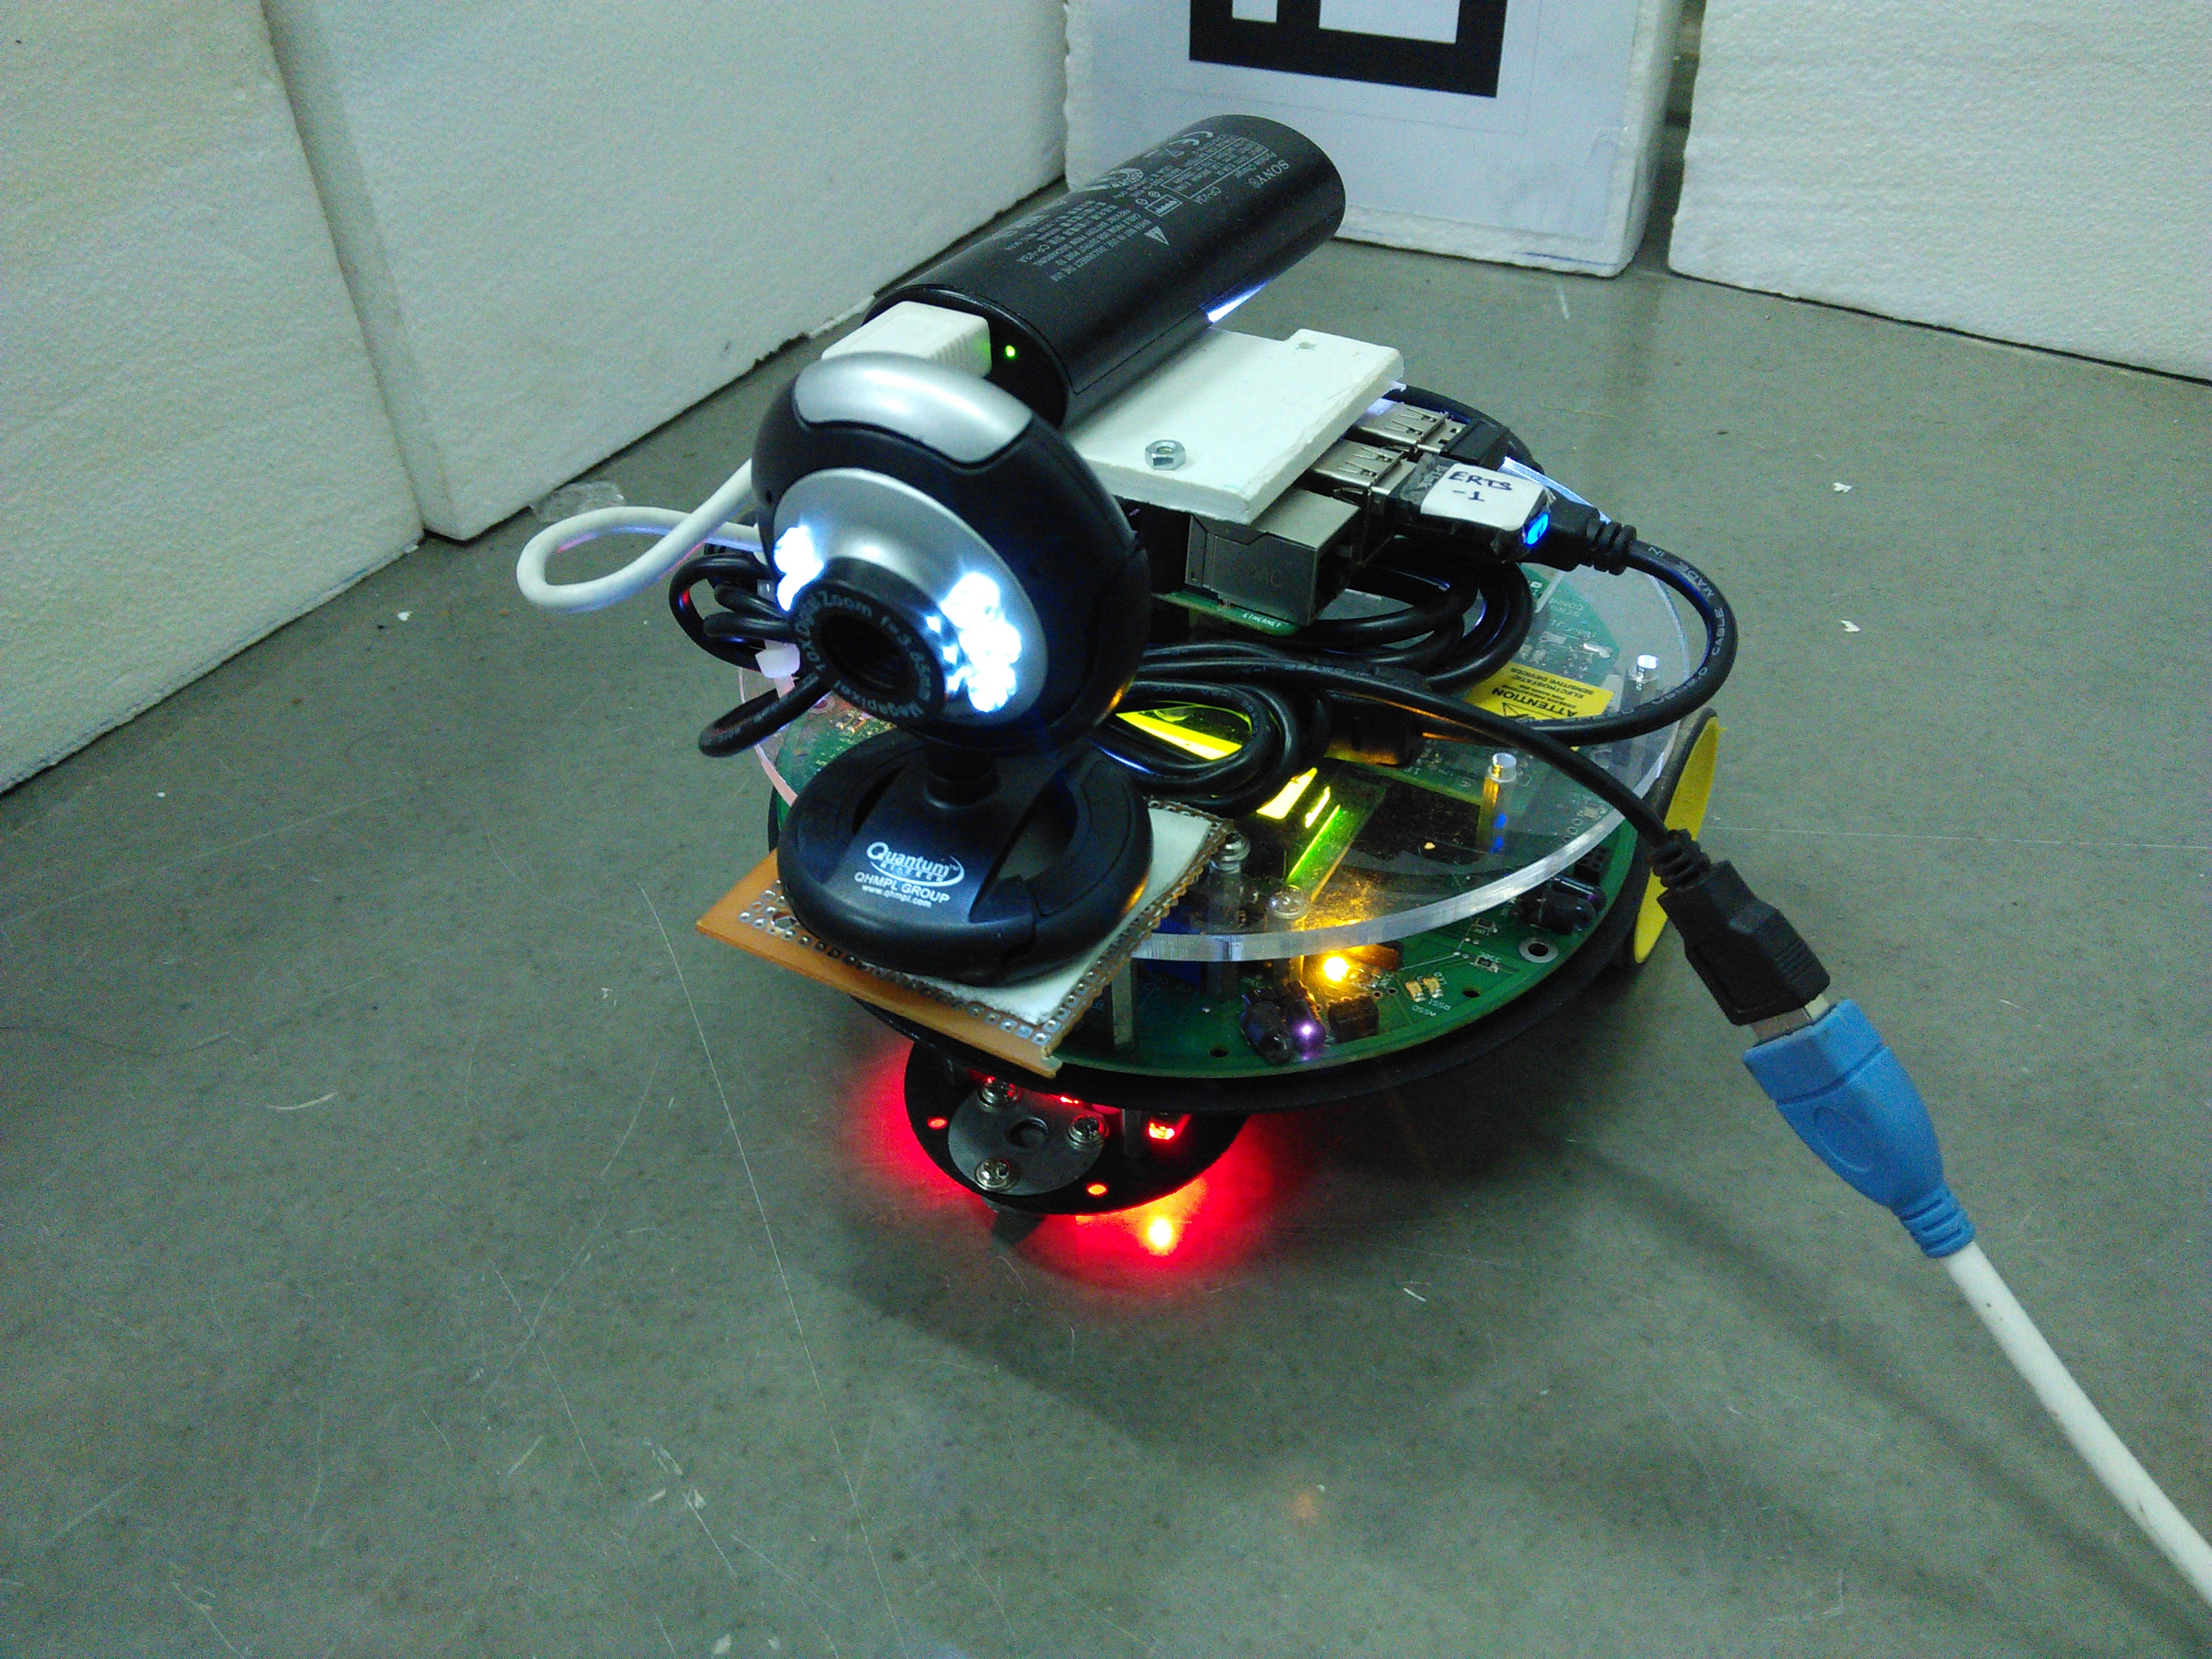
\includegraphics[width = 9cm]{Bot.jpg}

\section{Things to do:}\label{things-to-do}

\begin{itemize}
\tightlist
\item
  Connect the Raspi to the power bank and connect a HDMI cable. Once you
  have entered the GUI of the Raspi, type \texttt{ifconfig} in the
  terminal and note down the IP address of the network to which the
  wireless adapter is connected to.
\item
  Open MobaXterm on your PC and enter `ssh -x pi@192.168.1.119'
  considering the IP address is 192.168.1.119.
\item
  Once connected you can access the code on the Raspi.
\end{itemize}

\section{Code}\label{code}

Code to be run on the Raspi. This code will act as the client and send
data to the server.

\begin{Shaded}
\begin{Highlighting}[]
      \CommentTok{"""}
\CommentTok{     """}
\NormalTok{Code }\ControlFlowTok{for} \NormalTok{localizing a robot }\ControlFlowTok{with} \NormalTok{Aruco markers.}

\NormalTok{Authors: Niharika Jayanthi, Dheeraj Kamath}
\NormalTok{Project: Marker}\OperatorTok{-}\NormalTok{based Localization}
\NormalTok{Mentor: Sanam Shakya}

\NormalTok{Main functions:}

\NormalTok{Global variables:}

\CommentTok{"""}

\CommentTok{#Imports}

\CommentTok{import cv2}
\CommentTok{import socket}
\CommentTok{import numpy as np}
\CommentTok{import math}



\CommentTok{#Global variables}

\CommentTok{MAX_MARKERS = 4}

\CommentTok{mark_detect = [0, 0, 0, 0]}
\CommentTok{    }
\CommentTok{objp = np.zeros((1*4,3), np.float32)}

\CommentTok{objp[1,1] = 1}
\CommentTok{objp[2,0] = 1}
\CommentTok{objp[2,1] = 1}
\CommentTok{objp[3,0] = 1}

\CommentTok{objp = objp * 105}
\CommentTok{#(700/9.605116)}

\CommentTok{count = 0}

\CommentTok{s = socket.socket(socket.AF_INET, socket.SOCK_STREAM)}
\CommentTok{port = 7000}

\CommentTok{server_ip = '192.168.1.104'}

\CommentTok{s.connect((server_ip, port))}
\CommentTok{print "Connected to server"}


\CommentTok{#Helper functions}

\CommentTok{def is_aruco_present(img1):}
\CommentTok{    """}
    \OperatorTok{*} \NormalTok{Function Name:    is_aruco_present}
    \OperatorTok{*} \NormalTok{Input:        Image captured}
    \OperatorTok{*} \NormalTok{Output:       Returns the }\BuiltInTok{set} \NormalTok{of corner points of the marker }\OperatorTok{in} \NormalTok{the}
                        \NormalTok{image.}
    \OperatorTok{*} \NormalTok{Logic:            Takes the }\BuiltInTok{input} \NormalTok{image }\OperatorTok{and} \NormalTok{finds the contour having four points }\OperatorTok{and} \NormalTok{of specified area. }
    \OperatorTok{*} \NormalTok{Example Call: is_aruco_present()}
    \CommentTok{"""}

\CommentTok{    i = 0}
\CommentTok{    aruco_points = []}
\CommentTok{    gray1 = cv2.cvtColor(img1, cv2.COLOR_BGR2GRAY)}
\CommentTok{    ret, thresh1 = cv2.threshold(gray1, 175,255, cv2.THRESH_BINARY_INV+ cv2.THRESH_OTSU)}
\CommentTok{    img = thresh1.copy()}
\CommentTok{    kernel = np.ones((5,5), np.uint8)}
\CommentTok{    open1 = cv2.morphologyEx(thresh1, cv2.MORPH_OPEN, kernel)}
\CommentTok{    median1 = cv2.medianBlur(open1, 5)}
\CommentTok{    c1, h1 = cv2.findContours(thresh1, cv2.RETR_EXTERNAL, cv2.CHAIN_APPROX_SIMPLE)}
\CommentTok{    for c in c1:}
\CommentTok{        k = cv2.isContourConvex(c)     #Check for convexity, removes unwanted curved contours}
\CommentTok{        if k == True:}
\CommentTok{            i = i +1}
\CommentTok{            continue}
\CommentTok{        elif k == False:}
\CommentTok{            e2 = 0.1*cv2.arcLength(c, True)}
\CommentTok{            a2 = cv2.approxPolyDP(c, e2, True)}
\CommentTok{            print "a2 = ", a2, "\textbackslash{}n", "e2 =", e2}
\CommentTok{            if len(a2)== 4:}
\CommentTok{                x = a2[0,0,1]-a2[2,0,1] }
\CommentTok{                y = a2[2,0,0]-a2[0,0,0]}
\CommentTok{                if x < 0:}
\CommentTok{                    x = x * (-1)      #Converting to unsigned int}
\CommentTok{                if y < 0:}
\CommentTok{                    y = y * (-1)      #Converting to unsigned int}
\CommentTok{                if  10 < e2 < 100:              #45-60cm}
\CommentTok{                    print "Contour Id : ",i,"length of array =", len(a2), "\textbackslash{}n""\textbackslash{}n", a2}
\CommentTok{                    print x-y}
\CommentTok{                    if -50 < x-y < 50:  # Without tilt}
\CommentTok{                        aruco_points = a2}
\CommentTok{                        cv2.drawContours(img1, c1, i, (0,255,0), 2)}
\CommentTok{                        cv2.imshow('img',img1)}
\CommentTok{                        cv2.waitKey(500)}
\CommentTok{                        cv2.destroyAllWindows()}
\CommentTok{                        return aruco_points, '1'  # Flag values can be changed as per convenience}
\CommentTok{                    elif -80 < x-y < 80:  #with tilt}
\CommentTok{                        aruco_points = a2}
\CommentTok{                        cv2.drawContours(img1, c1, i, (0,255,0), 2)}
\CommentTok{                        cv2.imshow('img',img1)}
\CommentTok{                        cv2.waitKey(500)}
\CommentTok{                        cv2.destroyAllWindows()}
\CommentTok{                        return aruco_points, '1'}
\CommentTok{                elif 100 < x-y < 200:}
\CommentTok{                    print "Contour Id : ",i,"length of array =", len(a2), "\textbackslash{}n""\textbackslash{}n", a2}
\CommentTok{                    print x-y}
\CommentTok{                    if -10 < x-y < 10:}
\CommentTok{                        aruco_points = a2}
\CommentTok{                        cv2.drawContours(img1, c1, i, (0,255,0), 2)}
\CommentTok{                        cv2.imshow('img',img1)}
\CommentTok{                        cv2.waitKey(500)}
\CommentTok{                        cv2.destroyAllWindows()}
\CommentTok{                        return aruco_points, '1'}
\CommentTok{        i = i + 1}
\CommentTok{                                                        }
\CommentTok{            }
\CommentTok{                        }
\CommentTok{    if aruco_points == []:}
\CommentTok{        return '-1', '-1'}
\CommentTok{            }

\CommentTok{    }
\CommentTok{    }
\CommentTok{def Perspective(aruco_points,img_name):}
\CommentTok{    """}
    \OperatorTok{*} \NormalTok{Function Name:    Perspective}
    \OperatorTok{*} \NormalTok{Input:        A numpy array }\ControlFlowTok{with} \NormalTok{four points }\OperatorTok{and} \NormalTok{name of an image}
    \OperatorTok{*} \NormalTok{Output:       Returns the image after performing perspective transform}
                        \NormalTok{on it}
    \OperatorTok{*} \NormalTok{Logic:        If the image points have a varied difference between the points, it means the image }\OperatorTok{is}
                        \NormalTok{tilted }\OperatorTok{and} \NormalTok{thus the points are mapped to proper }\BuiltInTok{set} \NormalTok{of points }\OperatorTok{and} \NormalTok{made parallel to the                                  }
                        \NormalTok{image plane.  }
    \OperatorTok{*} \NormalTok{Example Call: Perspective(points, }\StringTok{"Marker.jpg"}\NormalTok{)}
    \CommentTok{"""}
\CommentTok{    img = cv2.imread(img_name)}
\CommentTok{    a1 = aruco_points}
\CommentTok{    print aruco_points}
\CommentTok{    if a1[0,0,0]>a1[1,0,0]:}
\CommentTok{        pts1 = np.float32([a1[1,0], a1[2,0], a1[3,0], a1[0,0]])}
\CommentTok{        pts2 = np.float32([[0,0], [0,300], [300,300], [300,0]])}

\CommentTok{    elif a1[0,0,0] < a1[1,0,0] :}
\CommentTok{        pts1 = np.float32([a1[0,0], a1[1,0], a1[2,0], a1[3,0]])}
\CommentTok{        pts2 = np.float32([[0,0], [0,300], [300,300], [300,0]])}
\CommentTok{    print pts1}
\CommentTok{    print pts2}
\CommentTok{    M = cv2.getPerspectiveTransform(pts1,pts2)}

\CommentTok{    dst = cv2.warpPerspective(img,M,(300,300))}
\CommentTok{    per_img = dst.copy()}
\CommentTok{    cv2.imshow("Perspective",dst)}
\CommentTok{    cv2.waitKey(500)}
\CommentTok{    cv2.destroyAllWindows()}
\CommentTok{    resize = cv2.resize(per_img, (399,399), interpolation = cv2.INTER_CUBIC)}
\CommentTok{    #Grid box}
\CommentTok{    dx, dy = 57,57}

\CommentTok{    # Custom (rgb) grid color}
\CommentTok{    grid_color = [0,0,255]}

\CommentTok{    # Modify the image to include the grid}
\CommentTok{    resize[:,::dy,:] = grid_color}
\CommentTok{    resize[::dx,:,:] = grid_color}
\CommentTok{    aruco = resize[57:342, 57:342]}
\CommentTok{    cv2.imshow("grid",aruco)}
\CommentTok{    cv2.waitKey(500)}
\CommentTok{    cv2.destroyAllWindows()}
\CommentTok{    ret, thresh= cv2.threshold(aruco, 127,255, cv2.THRESH_BINARY)}
\CommentTok{    g2 = cv2.cvtColor(thresh, cv2.COLOR_BGR2GRAY)}
\CommentTok{    return g2, pts1}




\CommentTok{def Crop(aruco_points,img_name):}
\CommentTok{"""}
    \OperatorTok{*} \NormalTok{Function Name:    Crop}
    \OperatorTok{*} \NormalTok{Input:        A numpy array }\ControlFlowTok{with} \NormalTok{four points }\OperatorTok{and} \NormalTok{name of an image}
    \OperatorTok{*} \NormalTok{Output:       Returns the image after performing a refined perspective transform.}
                        \NormalTok{on it}
    \OperatorTok{*} \NormalTok{Logic:        If the image points have a varied difference between the points, it means the image }\OperatorTok{is}
                        \NormalTok{tilted }\OperatorTok{and} \NormalTok{thus the points are mapped to defined }\BuiltInTok{set} \NormalTok{of points }\OperatorTok{and} \NormalTok{made parallel to the                                  }
                        \NormalTok{image plane.  }
    \OperatorTok{*} \NormalTok{Example Call: Crop(points, }\StringTok{"Marker.jpg"}\NormalTok{)}
    \NormalTok{img }\OperatorTok{=} \NormalTok{cv2.imread(img_name)}
    \NormalTok{a1 }\OperatorTok{=} \NormalTok{aruco_points}
    \BuiltInTok{print} \NormalTok{aruco_points}
    \NormalTok{lx }\OperatorTok{=} \OperatorTok{-}\DecValTok{999}
    \NormalTok{ly }\OperatorTok{=} \OperatorTok{-}\DecValTok{999}
    \NormalTok{sx }\OperatorTok{=} \DecValTok{999}
    \NormalTok{sy }\OperatorTok{=} \DecValTok{999}
    \ControlFlowTok{for} \NormalTok{i }\OperatorTok{in} \BuiltInTok{range}\NormalTok{(}\DecValTok{0}\NormalTok{,}\DecValTok{4}\NormalTok{):}
        \ControlFlowTok{if} \NormalTok{a1[i,}\DecValTok{0}\NormalTok{,}\DecValTok{0}\NormalTok{] }\OperatorTok{>} \NormalTok{lx :}
            \NormalTok{lx }\OperatorTok{=} \NormalTok{a1[i,}\DecValTok{0}\NormalTok{,}\DecValTok{0}\NormalTok{]}
    \BuiltInTok{print} \NormalTok{lx}

    \ControlFlowTok{for} \NormalTok{i }\OperatorTok{in} \BuiltInTok{range}\NormalTok{(}\DecValTok{0}\NormalTok{,}\DecValTok{4}\NormalTok{):}
        \ControlFlowTok{if} \NormalTok{a1[i,}\DecValTok{0}\NormalTok{,}\DecValTok{0}\NormalTok{] }\OperatorTok{<} \NormalTok{sx:}
            \NormalTok{sx }\OperatorTok{=} \NormalTok{a1[i,}\DecValTok{0}\NormalTok{,}\DecValTok{0}\NormalTok{]}
    \BuiltInTok{print} \NormalTok{sx }

    \ControlFlowTok{for} \NormalTok{i }\OperatorTok{in} \BuiltInTok{range}\NormalTok{(}\DecValTok{0}\NormalTok{,}\DecValTok{4}\NormalTok{):}
        \ControlFlowTok{if} \NormalTok{a1[i,}\DecValTok{0}\NormalTok{,}\DecValTok{1}\NormalTok{] }\OperatorTok{>} \NormalTok{ly:}
            \NormalTok{ly }\OperatorTok{=} \NormalTok{a1[i,}\DecValTok{0}\NormalTok{,}\DecValTok{1}\NormalTok{]}
    \BuiltInTok{print} \NormalTok{ly}
    \ControlFlowTok{for} \NormalTok{i }\OperatorTok{in} \BuiltInTok{range}\NormalTok{(}\DecValTok{0}\NormalTok{,}\DecValTok{4}\NormalTok{):}
        \ControlFlowTok{if} \NormalTok{a1[i,}\DecValTok{0}\NormalTok{,}\DecValTok{1}\NormalTok{] }\OperatorTok{<} \NormalTok{sy:}
            \NormalTok{sy }\OperatorTok{=} \NormalTok{a1[i,}\DecValTok{0}\NormalTok{,}\DecValTok{1}\NormalTok{]}
    \BuiltInTok{print} \NormalTok{sy}
    \CommentTok{'''}
\CommentTok{    for i in range(0,4):}
\CommentTok{        if 0 < a1[i,0,0] - sx < 10:}
\CommentTok{            if a[i, 0, 1] == sy:}
\CommentTok{                a1[0,0] = [a1[i, 0, 0], sy]}
\CommentTok{                a1[1,0] = [sx,}
\CommentTok{    '''}
    \NormalTok{pts1 }\OperatorTok{=} \NormalTok{np.float32([[sx,sy],[sx,ly],[lx,ly],[lx,sy]])}
    \NormalTok{pts2 }\OperatorTok{=} \NormalTok{np.float32([[}\DecValTok{0}\NormalTok{,}\DecValTok{0}\NormalTok{],[}\DecValTok{0}\NormalTok{,}\DecValTok{300}\NormalTok{],[}\DecValTok{300}\NormalTok{,}\DecValTok{300}\NormalTok{],[}\DecValTok{300}\NormalTok{,}\DecValTok{0}\NormalTok{]])}
    \BuiltInTok{print} \NormalTok{pts1}
    \BuiltInTok{print} \NormalTok{pts2}
    \NormalTok{M }\OperatorTok{=} \NormalTok{cv2.getPerspectiveTransform(pts1,pts2)}

    \NormalTok{dst }\OperatorTok{=} \NormalTok{cv2.warpPerspective(img,M,(}\DecValTok{300}\NormalTok{,}\DecValTok{300}\NormalTok{))}
    \NormalTok{per_img }\OperatorTok{=} \NormalTok{dst.copy()}
    \NormalTok{cv2.imshow(}\StringTok{"crop"}\NormalTok{,dst)}
    \NormalTok{cv2.waitKey(}\DecValTok{500}\NormalTok{)}
    \NormalTok{cv2.destroyAllWindows()}
    \NormalTok{resize }\OperatorTok{=} \NormalTok{cv2.resize(per_img, (}\DecValTok{399}\NormalTok{,}\DecValTok{399}\NormalTok{), interpolation }\OperatorTok{=} \NormalTok{cv2.INTER_CUBIC)}
    \CommentTok{#Grid box}
    \NormalTok{dx, dy }\OperatorTok{=} \DecValTok{57}\NormalTok{,}\DecValTok{57}

    \CommentTok{# Custom (rgb) grid color}
    \NormalTok{grid_color }\OperatorTok{=} \NormalTok{[}\DecValTok{0}\NormalTok{,}\DecValTok{0}\NormalTok{,}\DecValTok{255}\NormalTok{]}

    \CommentTok{# Modify the image to include the grid}
    \NormalTok{resize[:,::dy,:] }\OperatorTok{=} \NormalTok{grid_color}
    \NormalTok{resize[::dx,:,:] }\OperatorTok{=} \NormalTok{grid_color}
    \NormalTok{aruco }\OperatorTok{=} \NormalTok{resize[}\DecValTok{57}\NormalTok{:}\DecValTok{342}\NormalTok{, }\DecValTok{57}\NormalTok{:}\DecValTok{342}\NormalTok{]}
    \NormalTok{cv2.imshow(}\StringTok{"grid"}\NormalTok{,aruco)}
    \NormalTok{cv2.waitKey(}\DecValTok{500}\NormalTok{)}
    \NormalTok{cv2.destroyAllWindows()}
    \NormalTok{ret, thresh}\OperatorTok{=} \NormalTok{cv2.threshold(aruco, }\DecValTok{127}\NormalTok{,}\DecValTok{255}\NormalTok{, cv2.THRESH_BINARY)}
    \NormalTok{g2 }\OperatorTok{=} \NormalTok{cv2.cvtColor(thresh, cv2.COLOR_BGR2GRAY)}
    \ControlFlowTok{return} \NormalTok{g2, pts1}

\KeywordTok{def} \NormalTok{findArucoID(marker_img):}
    \CommentTok{"""}
\CommentTok{    * Function Name:    findArucoID}
\CommentTok{    * Input:        An image of Aruco marker.}
\CommentTok{    * Output:       Returns an integer value that represents the ID of the}
\CommentTok{                        Aruco marker}
\CommentTok{    * Logic:        The second and fourth columns from the Aruco marker are}
\CommentTok{                        analyzed. If the pixel value in the grid cell is 0}
\CommentTok{                        (black), it is taken as 0. If it is 255(white), it is}
\CommentTok{                        considered as 1. The binary number is generated by}
\CommentTok{                        reading in a top-bottom, left-right manner.}
\CommentTok{    * Example Call: findArucoID(img)}
\CommentTok{    """}

    \NormalTok{height }\OperatorTok{=} \DecValTok{57}
    \NormalTok{width }\OperatorTok{=} \DecValTok{57}
    \NormalTok{ret_val }\OperatorTok{=} \DecValTok{0}
    \NormalTok{cv2.imshow(}\StringTok{"aruco"}\NormalTok{, marker_img)}
    \NormalTok{cv2.waitKey(}\DecValTok{500}\NormalTok{)}
    \NormalTok{cv2.destroyAllWindows()}
    \ControlFlowTok{for} \NormalTok{i }\OperatorTok{in} \BuiltInTok{range}\NormalTok{(}\DecValTok{5}\NormalTok{):}
        \ControlFlowTok{for} \NormalTok{y }\OperatorTok{in} \NormalTok{(}\DecValTok{1}\NormalTok{, }\DecValTok{3}\NormalTok{):}
            \NormalTok{px1 }\OperatorTok{=} \NormalTok{marker_img[height}\OperatorTok{*}\NormalTok{i }\OperatorTok{+} \DecValTok{29}\NormalTok{, y }\OperatorTok{*} \NormalTok{width }\OperatorTok{+} \NormalTok{width}\OperatorTok{/}\DecValTok{2}\NormalTok{]}
            \ControlFlowTok{if} \NormalTok{px1 }\OperatorTok{==} \DecValTok{255}\NormalTok{:}
                \NormalTok{val }\OperatorTok{=} \DecValTok{1}
                \CommentTok{#binary.append(val)}
            \ControlFlowTok{else}\NormalTok{:}
                \NormalTok{val }\OperatorTok{=} \DecValTok{0}
                \CommentTok{#binary.append(val)}
            \NormalTok{ret_val }\OperatorTok{=} \DecValTok{2} \OperatorTok{*} \NormalTok{ret_val }\OperatorTok{+} \NormalTok{val}
    \CommentTok{#print "Binary", binary, ret_val}
    \ControlFlowTok{return} \NormalTok{ret_val}


\KeywordTok{def} \NormalTok{sendPoints(x, y, t, t1, markerID):}
    \CommentTok{"""}
\CommentTok{    * Function Name:    sendPoints}
\CommentTok{    * Input:        The (x,y) coordinates of a point, angle, t, which is the}
\CommentTok{                        rotation angle and the ID(integer) of the marker whose}
\CommentTok{                        points are being sent.}
\CommentTok{    * Output:       Sends a message to the server containing the information}
\CommentTok{                        from the input}
\CommentTok{    * Logic:        A TCP message is sent to the server through socket}
\CommentTok{                        programming.}
\CommentTok{    * Example Call: sendPoints(269, 346, 1.11812, 34)}
\CommentTok{    """}
    \KeywordTok{global} \NormalTok{s}

    
    \NormalTok{msg }\OperatorTok{=} \BuiltInTok{str}\NormalTok{(x) }\OperatorTok{+} \StringTok{" "} \OperatorTok{+} \BuiltInTok{str}\NormalTok{(y) }\OperatorTok{+} \StringTok{" "} \OperatorTok{+} \BuiltInTok{str}\NormalTok{(t) }\OperatorTok{+} \StringTok{" "}\OperatorTok{+}\BuiltInTok{str}\NormalTok{(t1) }\OperatorTok{+} \StringTok{" "}\OperatorTok{+} \BuiltInTok{str}\NormalTok{(markerID)}
    \BuiltInTok{print} \StringTok{"message sent"}
        

    \NormalTok{s.send(msg)}
    


\KeywordTok{def} \NormalTok{getProperties(points):}
    \CommentTok{"""}
\CommentTok{    * Function Name:    getProperties}
\CommentTok{    * Input:        A set of four points of the corners of aruco markers.}
\CommentTok{                        These points can be obtained from is_aruco_present()}
\CommentTok{                        function.}
\CommentTok{    * Output:       -}
\CommentTok{    * Logic:        The Perspective-n-Point problem is solved by Ransac}
\CommentTok{                        algorithm. We obtain the translation and rotation}
\CommentTok{                        vectors through this function.}
\CommentTok{    * Example Call: getProperties(points)}
\CommentTok{    """}

    \KeywordTok{global} \NormalTok{objp}
    
    \CommentTok{# Arrays to store object points and image points from all the images.}
    \NormalTok{objpoints }\OperatorTok{=} \NormalTok{objp}
    \BuiltInTok{print} \StringTok{"OBJP"}\NormalTok{, objpoints}
    
    \NormalTok{imgpoints }\OperatorTok{=} \NormalTok{points}

    \CommentTok{#imgpoints = np.array(imgpoints)}
    \BuiltInTok{print} \StringTok{"IMGP"}\NormalTok{, imgpoints}

    \NormalTok{mtx }\OperatorTok{=} \NormalTok{np.load(}\StringTok{'matrix.npy'}\NormalTok{)}
    \NormalTok{dist }\OperatorTok{=} \NormalTok{np.load(}\StringTok{'distortion.npy'}\NormalTok{)}

    \NormalTok{rvec, tvec, inliers }\OperatorTok{=} \NormalTok{cv2.solvePnPRansac(objpoints, imgpoints, mtx, dist)}
    \BuiltInTok{print} \StringTok{"Rvec}\CharTok{\textbackslash{}n}\StringTok{"}\NormalTok{, rvec}
    \BuiltInTok{print} \StringTok{"}\CharTok{\textbackslash{}n}\StringTok{Tvec"}\NormalTok{, tvec}

    \NormalTok{x }\OperatorTok{=} \NormalTok{tvec[}\DecValTok{0}\NormalTok{][}\DecValTok{0}\NormalTok{]}
    \NormalTok{y }\OperatorTok{=} \NormalTok{tvec[}\DecValTok{2}\NormalTok{][}\DecValTok{0}\NormalTok{]}

    \NormalTok{dst, jacobian }\OperatorTok{=} \NormalTok{cv2.Rodrigues(rvec)}

    \BuiltInTok{print} \StringTok{"Rot Matrix"}\NormalTok{, dst}

    \NormalTok{t }\OperatorTok{=} \NormalTok{math.asin(}\OperatorTok{-}\NormalTok{dst[}\DecValTok{0}\NormalTok{][}\DecValTok{2}\NormalTok{])}
    \NormalTok{t1 }\OperatorTok{=} \NormalTok{math.acos(dst[}\DecValTok{0}\NormalTok{][}\DecValTok{0}\NormalTok{])}

    \ControlFlowTok{return} \NormalTok{x, y, t, t1}


\KeywordTok{def} \NormalTok{Video(}\VariableTok{True}\NormalTok{):}
    \CommentTok{"""}
\CommentTok{    * Function Name:    Video}
\CommentTok{    * Input:        -}
\CommentTok{    * Output:           Analyzes and detects markers till all markers are}
\CommentTok{                        detected.}
\CommentTok{    * Logic:        It runs through a infinite loop checking}
\CommentTok{                        every frame for markers. If marker is obtained,}
\CommentTok{                        it increments a count, else, next frame is analyzed.}
\CommentTok{                        This process is continued till all the markers are}
\CommentTok{                        detected.}
\CommentTok{    * Example Call: Video(True)}
\CommentTok{    """}
    \KeywordTok{global} \NormalTok{count,s, mark_detect}
    \NormalTok{cap }\OperatorTok{=} \NormalTok{cv2.VideoCapture(}\DecValTok{1}\NormalTok{)}

    \ControlFlowTok{while}\NormalTok{(}\VariableTok{True}\NormalTok{):}
        \NormalTok{ret, frame }\OperatorTok{=} \NormalTok{cap.read()}
        \NormalTok{cv2.imshow(}\StringTok{"Video"}\NormalTok{, frame)}
        \NormalTok{cv2.waitKey(}\DecValTok{500}\NormalTok{)}
        \NormalTok{aruco_points, flag }\OperatorTok{=} \NormalTok{is_aruco_present(frame)}
        \CommentTok{#cv2.imshow("Captured", frame)}
        \ControlFlowTok{if} \NormalTok{flag }\OperatorTok{!=} \StringTok{'-1'}\NormalTok{:}
            \NormalTok{img_name }\OperatorTok{=} \StringTok{"Marker.jpg"}
            \NormalTok{cv2.imwrite(img_name, frame)}
            \CommentTok{#count = count + 1}
            \ControlFlowTok{if} \NormalTok{flag }\OperatorTok{==} \StringTok{'1'}\NormalTok{:}
                \NormalTok{p_img, pts }\OperatorTok{=} \NormalTok{Crop(aruco_points, img_name)}
            \ControlFlowTok{elif} \NormalTok{flag }\OperatorTok{==} \StringTok{'2'}\NormalTok{:}
                \NormalTok{p_img, pts }\OperatorTok{=} \NormalTok{Perspective(aruco_points, img_name)}
            \NormalTok{m_id }\OperatorTok{=} \NormalTok{findArucoID(p_img)}
            \ControlFlowTok{if} \NormalTok{(m_id }\OperatorTok{==} \DecValTok{65} \OperatorTok{and} \NormalTok{mark_detect[}\DecValTok{0}\NormalTok{] }\OperatorTok{==} \DecValTok{0}\NormalTok{):}
                \NormalTok{mark_detect[}\DecValTok{0}\NormalTok{] }\OperatorTok{=} \DecValTok{1}
            \ControlFlowTok{elif} \NormalTok{(m_id }\OperatorTok{==} \DecValTok{796} \OperatorTok{and} \NormalTok{mark_detect[}\DecValTok{1}\NormalTok{] }\OperatorTok{==} \DecValTok{0}\NormalTok{):}
                \NormalTok{mark_detect[}\DecValTok{1}\NormalTok{] }\OperatorTok{=} \DecValTok{1}
            \ControlFlowTok{elif} \NormalTok{(m_id }\OperatorTok{==} \DecValTok{500} \OperatorTok{and} \NormalTok{mark_detect[}\DecValTok{2}\NormalTok{] }\OperatorTok{==} \DecValTok{0}\NormalTok{):}
                \NormalTok{mark_detect[}\DecValTok{2}\NormalTok{] }\OperatorTok{=} \DecValTok{1}
            \ControlFlowTok{elif} \NormalTok{(m_id }\OperatorTok{==} \DecValTok{250} \OperatorTok{and} \NormalTok{mark_detect[}\DecValTok{3}\NormalTok{] }\OperatorTok{==} \DecValTok{0}\NormalTok{):}
                \NormalTok{mark_detect[}\DecValTok{3}\NormalTok{] }\OperatorTok{=} \DecValTok{1}
            \ControlFlowTok{else}\NormalTok{:}
                \ControlFlowTok{continue}
            \NormalTok{count }\OperatorTok{=} \NormalTok{count }\OperatorTok{+} \DecValTok{1}
            \NormalTok{x, y, t, t1 }\OperatorTok{=} \NormalTok{getProperties(pts)}
            \ControlFlowTok{if} \NormalTok{(x }\OperatorTok{==} \FloatTok{0.0} \OperatorTok{and} \NormalTok{y }\OperatorTok{==} \FloatTok{0.0}\NormalTok{):}
                \NormalTok{count }\OperatorTok{=} \NormalTok{count }\OperatorTok{-} \DecValTok{1}
                \ControlFlowTok{if} \NormalTok{(m_id }\OperatorTok{==} \DecValTok{65} \OperatorTok{and} \NormalTok{mark_detect[}\DecValTok{0}\NormalTok{] }\OperatorTok{==} \DecValTok{1}\NormalTok{):}
                    \NormalTok{mark_detect[}\DecValTok{0}\NormalTok{] }\OperatorTok{=} \DecValTok{0}
                \ControlFlowTok{elif} \NormalTok{(m_id }\OperatorTok{==} \DecValTok{796} \OperatorTok{and} \NormalTok{mark_detect[}\DecValTok{1}\NormalTok{] }\OperatorTok{==} \DecValTok{1}\NormalTok{):}
                    \NormalTok{mark_detect[}\DecValTok{1}\NormalTok{] }\OperatorTok{=} \DecValTok{0}
                \ControlFlowTok{elif} \NormalTok{(m_id }\OperatorTok{==} \DecValTok{500} \OperatorTok{and} \NormalTok{mark_detect[}\DecValTok{2}\NormalTok{] }\OperatorTok{==} \DecValTok{1}\NormalTok{):}
                    \NormalTok{mark_detect[}\DecValTok{2}\NormalTok{] }\OperatorTok{=} \DecValTok{0}
                \ControlFlowTok{elif} \NormalTok{(m_id }\OperatorTok{==} \DecValTok{250} \OperatorTok{and} \NormalTok{mark_detect[}\DecValTok{3}\NormalTok{] }\OperatorTok{==} \DecValTok{1}\NormalTok{):}
                    \NormalTok{mark_detect[}\DecValTok{3}\NormalTok{] }\OperatorTok{=} \DecValTok{0}
                \ControlFlowTok{continue}
                
            \NormalTok{sendPoints(x, y, t, t1, m_id)}
            \BuiltInTok{print} \StringTok{"X"}\NormalTok{, x, }\StringTok{"Y"}\NormalTok{, y, }\StringTok{"T"}\NormalTok{, t, }\StringTok{"T1"}\NormalTok{, t1,  }\StringTok{"ID"}\NormalTok{, m_id}
            \ControlFlowTok{if} \NormalTok{count }\OperatorTok{==} \NormalTok{MAX_MARKERS:}
                \BuiltInTok{print} \StringTok{"All detected"}
                \BuiltInTok{print} \StringTok{"Closing connection"}
                \ControlFlowTok{if} \NormalTok{cv2.waitKey(}\DecValTok{1}\NormalTok{) }\OperatorTok{==} \DecValTok{32}\NormalTok{: }\CommentTok{# Ascii for spacebar}
                    \NormalTok{s.send(}\StringTok{'q'}\NormalTok{)}
                \ControlFlowTok{break}
                        
                    
            

    \NormalTok{cap.release()}
    \NormalTok{cv2.waitKey(}\DecValTok{0}\NormalTok{)     }\CommentTok{# Escape sequence}
    \NormalTok{cv2.destroyAllWindows()}

\NormalTok{Video(}\VariableTok{True}\NormalTok{)}
\NormalTok{s.close()}
\end{Highlighting}
\end{Shaded}

The server will have the following code-

\begin{Shaded}
\begin{Highlighting}[]
\CommentTok{"""}
\CommentTok{This code receives and maps points}

\CommentTok{Authors: Niharika Jayanthi, Dheeraj Kamath}
\CommentTok{Project: Marker-based Localization}
\CommentTok{Mentor: Sanam Shakya}

\CommentTok{Main functions: draw_arena(), draw_marker(), draw_robot()}
\CommentTok{                getCoordinates(), get_socket()}

\CommentTok{Global variables: arena_length, arena_breadth, s, host, port, room_width}

\CommentTok{"""}
\ImportTok{import} \NormalTok{socket}
\ImportTok{import} \NormalTok{cv2}
\ImportTok{from} \NormalTok{matplotlib }\ImportTok{import} \NormalTok{pyplot }\ImportTok{as} \NormalTok{plt}
\ImportTok{import} \NormalTok{numpy }\ImportTok{as} \NormalTok{np}
\ImportTok{import} \NormalTok{math}


\CommentTok{#Define Globals}

\NormalTok{arena_length}\OperatorTok{=}\DecValTok{600}
\NormalTok{arena_breadth}\OperatorTok{=}\DecValTok{600}

\NormalTok{s }\OperatorTok{=} \NormalTok{socket.socket(socket.AF_INET, socket.SOCK_STREAM)}
\NormalTok{host }\OperatorTok{=} \NormalTok{socket.gethostname()}
\NormalTok{port }\OperatorTok{=} \DecValTok{7000}
\NormalTok{s.bind((host, port))}
\NormalTok{s.listen(}\DecValTok{2}\NormalTok{)}

\NormalTok{room_width }\OperatorTok{=} \DecValTok{1160}


\CommentTok{#Helper functions}

\KeywordTok{def} \NormalTok{draw_arena(img1):}
    \CommentTok{"""}
\CommentTok{    * Function Name:    draw_arena}
\CommentTok{    * Input:        Image to be drawn in}
\CommentTok{    * Output:       Modified image with arena drawn}
\CommentTok{    * Logic:        The arena lines are drawn one at a time, with a distance}
\CommentTok{                        of 50 units separating them.}
\CommentTok{    * Example Call: draw_arena(image)}
\CommentTok{    """}
    \CommentTok{# Draw a diagonal blue line with thickness of 5 px}
    \NormalTok{row_width }\OperatorTok{=} \DecValTok{50}
    \NormalTok{col_width }\OperatorTok{=}  \DecValTok{50}

    \CommentTok{#print arena_length/50}
    \ControlFlowTok{for} \NormalTok{i }\OperatorTok{in} \BuiltInTok{range}\NormalTok{(}\DecValTok{0}\NormalTok{, arena_length}\OperatorTok{/}\NormalTok{row_width):}
        \NormalTok{cv2.line(img1,(row_width,}\DecValTok{0}\NormalTok{),(row_width,arena_length),(}\DecValTok{0}\NormalTok{,}\DecValTok{0}\NormalTok{,}\DecValTok{0}\NormalTok{),}\DecValTok{1}\NormalTok{)}
        \NormalTok{cv2.line(img1,(}\DecValTok{0}\NormalTok{,col_width),(arena_breadth,col_width),(}\DecValTok{0}\NormalTok{,}\DecValTok{0}\NormalTok{,}\DecValTok{0}\NormalTok{),}\DecValTok{1}\NormalTok{)}
        \NormalTok{row_width}\OperatorTok{=}\NormalTok{row_width}\DecValTok{+50}
        \NormalTok{col_width}\OperatorTok{=}\NormalTok{col_width}\DecValTok{+50}
    
    
\KeywordTok{def} \NormalTok{draw_marker(}\BuiltInTok{id}\NormalTok{, img1):}
    \CommentTok{"""}
\CommentTok{    * Function Name:    draw_marker}
\CommentTok{    * Input:        Marker ID, image to be drawn in}
\CommentTok{    * Output:       Returns 1 if valid marker is drawn. Else, it returns -1.}
\CommentTok{    * Logic:        The marker id is checked for validity. If marker is}
\CommentTok{                        valid, it draws in fixed position and returns 1. Else,}
\CommentTok{                        it returns -1.}
\CommentTok{    * Example Call: draw_marker(65, image)}
\CommentTok{    """}
    \NormalTok{marker_width }\OperatorTok{=} \DecValTok{50}
    \NormalTok{marker_length }\OperatorTok{=} \DecValTok{50}
    
    \NormalTok{font }\OperatorTok{=} \NormalTok{cv2.FONT_HERSHEY_SIMPLEX}

    \ControlFlowTok{if} \BuiltInTok{id} \OperatorTok{==} \DecValTok{65}\NormalTok{:}
        \NormalTok{x }\OperatorTok{=} \DecValTok{0}
        \NormalTok{y }\OperatorTok{=} \DecValTok{0}
    \ControlFlowTok{elif} \BuiltInTok{id} \OperatorTok{==} \DecValTok{250}\NormalTok{:}
        \NormalTok{x }\OperatorTok{=} \DecValTok{550}
        \NormalTok{y }\OperatorTok{=} \DecValTok{0}
    \ControlFlowTok{elif} \BuiltInTok{id} \OperatorTok{==} \DecValTok{796}\NormalTok{:}
        \NormalTok{x }\OperatorTok{=} \DecValTok{0}
        \NormalTok{y }\OperatorTok{=} \DecValTok{550}
    \ControlFlowTok{elif} \BuiltInTok{id} \OperatorTok{==} \DecValTok{500}\NormalTok{:}
        \NormalTok{x }\OperatorTok{=} \DecValTok{550}
        \NormalTok{y }\OperatorTok{=} \DecValTok{550}
    \ControlFlowTok{else}\NormalTok{:}
        \ControlFlowTok{return} \StringTok{'-1'}
    
    \NormalTok{cv2.rectangle(img1,(x,y),(x}\OperatorTok{+}\NormalTok{marker_width,y}\OperatorTok{+}\NormalTok{marker_length),(}\DecValTok{255}\NormalTok{,}\DecValTok{0}\NormalTok{,}\DecValTok{0}\NormalTok{,}\DecValTok{10}\NormalTok{),}\OperatorTok{-}\DecValTok{1}\NormalTok{)}
    \NormalTok{cv2.putText(img1,}\StringTok{'#'}\OperatorTok{+}\BuiltInTok{str}\NormalTok{(}\BuiltInTok{id}\NormalTok{),(x}\DecValTok{+10}\NormalTok{,y}\DecValTok{+30}\NormalTok{), font, }\FloatTok{0.5}\NormalTok{,(}\DecValTok{0}\NormalTok{,}\DecValTok{0}\NormalTok{,}\DecValTok{0}\NormalTok{),}\DecValTok{1}\NormalTok{)}

    \ControlFlowTok{return} \DecValTok{1}


\KeywordTok{def} \NormalTok{draw_robot(x, y, theta_radian, img1):}
    \CommentTok{"""}
\CommentTok{    * Function Name:    draw_robot()}
\CommentTok{    * Input:        x,y coordinates of the robot's position in map, angle}
\CommentTok{                        of inclination(theta) and image to be drawn in.}
\CommentTok{    * Output:       Modified image with the robot drawn in it and result is}
\CommentTok{                        displayed.}
\CommentTok{    * Logic:        The end point of the line is found by calculating a}
\CommentTok{                        rotation matrix and translating it. The robot is then}
\CommentTok{                        drawn as a circle and the line on the robot depicts}
\CommentTok{                        its orientation.}
\CommentTok{    * Example Call: draw_robot(250, 250, 45, image)}
\CommentTok{    """}
    \NormalTok{radius }\OperatorTok{=} \DecValTok{20}
    
    \NormalTok{rotation_matrix}\OperatorTok{=} \NormalTok{[[np.cos(theta_radian), }\OperatorTok{-}\NormalTok{np.sin(theta_radian)],}
                      \NormalTok{[np.sin(theta_radian), np.cos(theta_radian)]]}
    \NormalTok{R }\OperatorTok{=} \NormalTok{np.array(rotation_matrix)}
    \NormalTok{xy }\OperatorTok{=} \NormalTok{[[radius],[}\DecValTok{0}\NormalTok{]]}
    \NormalTok{xy }\OperatorTok{=} \NormalTok{np.array(xy)}
    \NormalTok{rotated_xy }\OperatorTok{=} \NormalTok{np.dot(R,xy)}

    \NormalTok{translation }\OperatorTok{=} \NormalTok{[[x],[y]]}
    \NormalTok{translation }\OperatorTok{=} \NormalTok{np.array(translation)}
    \NormalTok{trans_xy }\OperatorTok{=} \NormalTok{rotated_xy }\OperatorTok{+} \NormalTok{translation}

    \CommentTok{#Convert from floating point to integers}
    \NormalTok{x }\OperatorTok{=} \BuiltInTok{int}\NormalTok{(x)}
    \NormalTok{y }\OperatorTok{=} \BuiltInTok{int}\NormalTok{(y)}
    
    \NormalTok{cv2.circle(img1,(x,y), radius, (}\DecValTok{0}\NormalTok{,}\DecValTok{0}\NormalTok{,}\DecValTok{255}\NormalTok{), }\OperatorTok{-}\DecValTok{1}\NormalTok{)}

    \NormalTok{cv2.line(img1,(x,y),(trans_xy[}\DecValTok{0}\NormalTok{],trans_xy[}\DecValTok{1}\NormalTok{]),(}\DecValTok{0}\NormalTok{,}\DecValTok{0}\NormalTok{,}\DecValTok{0}\NormalTok{),}\DecValTok{2}\NormalTok{)}
    \NormalTok{cv2.imshow(}\StringTok{"Position"}\NormalTok{, img1)}
    \NormalTok{cv2.waitKey(}\DecValTok{1000}\NormalTok{)}


\KeywordTok{def} \NormalTok{getCoordinates(x, y, t, mID):}
    \CommentTok{"""}
\CommentTok{    * Function Name:    getCoordinates}
\CommentTok{    * Input:        x, y coordinates of point, angle t, marker ID}
\CommentTok{    * Output:       Returns new values of x, y and t.}
\CommentTok{    * Logic:        It compares the marker ID to a valid list of markers,}
\CommentTok{                        whose position in a room is already known to us and}
\CommentTok{                        returns the values of x,y and t according to the ID.}
\CommentTok{    * Example Call: getCoordinates(125, 235, 45, 500)}
\CommentTok{    """}

    \ControlFlowTok{if} \NormalTok{mID }\OperatorTok{==} \DecValTok{65}\NormalTok{:}
        \ControlFlowTok{return} \NormalTok{x, y, }\DecValTok{3}\OperatorTok{*}\NormalTok{math.pi}\OperatorTok{/}\DecValTok{2} \OperatorTok{-} \BuiltInTok{abs}\NormalTok{(t)}
    \ControlFlowTok{elif} \NormalTok{mID }\OperatorTok{==} \DecValTok{796}\NormalTok{:}
        \ControlFlowTok{return} \NormalTok{x, }\DecValTok{550} \OperatorTok{-} \NormalTok{y, math.pi}\OperatorTok{/}\DecValTok{2} \OperatorTok{+} \BuiltInTok{abs}\NormalTok{(t)}
    \ControlFlowTok{elif} \NormalTok{mID }\OperatorTok{==} \DecValTok{500}\NormalTok{:}
        \ControlFlowTok{return} \DecValTok{550} \OperatorTok{-} \NormalTok{x, }\DecValTok{550} \OperatorTok{-} \NormalTok{y, math.pi}\OperatorTok{/}\DecValTok{2} \OperatorTok{-} \BuiltInTok{abs}\NormalTok{(t)}
    \ControlFlowTok{elif} \NormalTok{mID }\OperatorTok{==} \DecValTok{250}\NormalTok{:}
        \ControlFlowTok{return} \DecValTok{550} \OperatorTok{-} \NormalTok{x, y, }\DecValTok{3} \OperatorTok{*} \NormalTok{math.pi}\OperatorTok{/}\DecValTok{2} \OperatorTok{+} \BuiltInTok{abs}\NormalTok{(t)}
    \ControlFlowTok{else}\NormalTok{:}
        \BuiltInTok{print} \StringTok{"Marker doen't match!"}
        \ControlFlowTok{return} \DecValTok{0}\NormalTok{, }\DecValTok{0}\NormalTok{, }\DecValTok{0}



\KeywordTok{def} \NormalTok{get_socket():}
    \CommentTok{"""}
\CommentTok{    * Function Name:    get_socket}
\CommentTok{    * Input:        -}
\CommentTok{    * Output:       -}
\CommentTok{    * Logic:        This function creates a TCP socket and receives}
\CommentTok{                        information from the client. This information includes}
\CommentTok{                        x, y coordinates of a marker, the angle t(calculated}
\CommentTok{                        with sine inverse), angle t1 (calculated as cosine}
\CommentTok{                        inverse) and the marker ID detected. These values are}
\CommentTok{                        passed to getCoordinates, which returns the x,y}
\CommentTok{                        values scaled to virtual map. Then, the marker/arena and}
\CommentTok{                        robot is drawn.}
\CommentTok{    * Example Call: get_socket()}
\CommentTok{    """}
    \KeywordTok{global} \NormalTok{s, first_msg, arena_M, cur_x, cur_y}

    \NormalTok{c, addr }\OperatorTok{=} \NormalTok{s.accept()}

    \ControlFlowTok{while} \VariableTok{True}\NormalTok{:}
        \NormalTok{msg }\OperatorTok{=} \NormalTok{c.recv(}\DecValTok{100}\NormalTok{)}
        \BuiltInTok{print} \StringTok{"Message received is"}\NormalTok{, msg}
        
        \ControlFlowTok{try}\NormalTok{:}
            \ControlFlowTok{if} \NormalTok{msg }\OperatorTok{==} \StringTok{'q'}\NormalTok{:}
                \BuiltInTok{print} \StringTok{"End of messages.}\CharTok{\textbackslash{}n}\StringTok{"}
                \ControlFlowTok{break}

            \NormalTok{x, y, t, t1, m_id }\OperatorTok{=} \NormalTok{msg.split()}
            \NormalTok{x }\OperatorTok{=} \BuiltInTok{float}\NormalTok{(x)}
            \NormalTok{y }\OperatorTok{=} \BuiltInTok{float}\NormalTok{(y)}
            \NormalTok{t }\OperatorTok{=} \BuiltInTok{float}\NormalTok{(t)}
            \NormalTok{t1 }\OperatorTok{=} \BuiltInTok{float}\NormalTok{(t1)}
            \NormalTok{m_id }\OperatorTok{=} \BuiltInTok{int}\NormalTok{(m_id)}

            \NormalTok{x }\OperatorTok{=} \DecValTok{600} \OperatorTok{*} \NormalTok{(x}\OperatorTok{/}\NormalTok{room_width)}
            \NormalTok{y }\OperatorTok{=} \DecValTok{600} \OperatorTok{*} \NormalTok{(y}\OperatorTok{/}\NormalTok{room_width)}
            
            \NormalTok{Rx }\OperatorTok{=} \BuiltInTok{abs}\NormalTok{(y }\OperatorTok{*} \NormalTok{math.cos(math.pi}\OperatorTok{/}\DecValTok{2} \OperatorTok{-} \NormalTok{t))}
            \NormalTok{Ry }\OperatorTok{=} \BuiltInTok{abs}\NormalTok{(y }\OperatorTok{*} \NormalTok{math.sin(math.pi}\OperatorTok{/}\DecValTok{2} \OperatorTok{-} \NormalTok{t))}
            \NormalTok{img_arena }\OperatorTok{=} \NormalTok{arena_M.copy()}
            \NormalTok{ret }\OperatorTok{=} \NormalTok{draw_marker(m_id, arena_M)}
            \ControlFlowTok{if} \NormalTok{ret }\OperatorTok{==} \StringTok{'-1'}\NormalTok{:}
                \BuiltInTok{print} \StringTok{"Marker not recognised."}
                
            \BuiltInTok{print} \StringTok{"X"}\NormalTok{, x, }\StringTok{"Y"}\NormalTok{, y, }\StringTok{"T"}\NormalTok{, t, }\StringTok{"T1"}\NormalTok{, t1, }\StringTok{"mID"}\NormalTok{, m_id}

            \BuiltInTok{print} \StringTok{"Rx"}\NormalTok{, Rx, }\StringTok{"Ry"}\NormalTok{, Ry}

            \NormalTok{mx, my, t }\OperatorTok{=} \NormalTok{getCoordinates(Rx, Ry, t, m_id)}

            \ControlFlowTok{if} \NormalTok{(mx,my,t) }\OperatorTok{==} \NormalTok{(}\DecValTok{0}\NormalTok{,}\DecValTok{0}\NormalTok{,}\DecValTok{0}\NormalTok{):}
                \BuiltInTok{print} \StringTok{"Invalid coordinates"}
                \ControlFlowTok{continue}
            \NormalTok{arena_copy }\OperatorTok{=} \NormalTok{arena_M.copy()}
            \NormalTok{draw_robot(mx, my, t, arena_copy)}
            
        \ControlFlowTok{except} \PreprocessorTok{ValueError}\NormalTok{:}
            \BuiltInTok{print} \StringTok{"Bad message!}\CharTok{\textbackslash{}n}\StringTok{"}
            \ControlFlowTok{break}

\CommentTok{# Create a black image}
\NormalTok{img }\OperatorTok{=} \NormalTok{np.ones((arena_length,arena_breadth,}\DecValTok{4}\NormalTok{), np.uint8)}\OperatorTok{*}\DecValTok{245}
\CommentTok{#img2 = np.ones((arena_length,arena_breadth,4), np.uint8)*255}

\NormalTok{draw_arena(img)}
\NormalTok{arena_M }\OperatorTok{=} \NormalTok{img}
\NormalTok{get_socket()}
\NormalTok{s.close()}

\CommentTok{#cv2.imshow("Map", arena_M)}
\NormalTok{cv2.waitKey(}\DecValTok{0}\NormalTok{)}
\NormalTok{cv2.destroyAllWindows()}
                                
\end{Highlighting}
\end{Shaded}

\section{Resources}
\begin{itemize}
	\item \href{https://github.com/eyantrainternship/eYSIP_2015_Marker_based_Robot_Localisation/blob/master/Task-7/Marker-based%20Localization/src/Server.py}{Server code - Github link}
	\item \href{https://github.com/eyantrainternship/eYSIP_2015_Marker_based_Robot_Localisation/blob/master/Task-7/Marker-based%20Localization/src/Client2.py}{Client code - Github link}
\end{itemize}

\end{document}
